\documentclass[crop,class=article]{standalone}
%----------------------------Preamble-------------------------------%
\usepackage{tikz}                       % Drawing/graphing tools.
\usetikzlibrary{arrows.meta}            % Latex and Stealth arrows.
%--------------------------Main Document----------------------------%
\begin{document}
    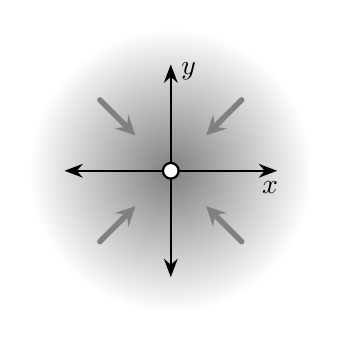
\begin{tikzpicture}[%
        scale=0.9,
        line width=1pt,
        line cap=round,
        >={Stealth[black]},
        every edge/.style={%
            draw=black,
            very thick
        },
        grayarrow/.style={%
            >=stealth,
            fill=gray,
            draw=gray,
            line width=0.7mm,
            ->
        }
    ]
        \filldraw[%
            even odd rule,
            inner color=gray,
            outer color=white,
            draw=white
        ] (0,0) circle (2);
        \draw[thick, <->] (-1.5,0)--(1.5,0);
        \draw[thick, <->] (0,-1.5)--(0,1.5);
        \draw[grayarrow] (1,1)--(0.5,0.5);
        \draw[grayarrow] (-1,-1)--(-0.5,-0.5);
        \draw[grayarrow] (1,-1)--(0.5,-0.5);
        \draw[grayarrow] (-1,1)--(-0.5,0.5);
        \node[%
            fill=white,
            circle,
            thick,
            draw,
            inner sep=2pt,
            outer sep=3pt
        ]
            at (0,0) (O) {};
        \node at (1.4,0) [below] {$x$};
        \node at (0,1.4) [right] {$y$};
    \end{tikzpicture}
\end{document}